\documentclass{article}
\usepackage{amsmath}
\usepackage{graphicx}
\begin{document}
\title{Coordinate Geometry Unit Exam: Question 37}
\author{Ana Bhattacharjee}
\date{\today}
\maketitle{}

\begin{center}
  The image of the garden is shown below.
  \begin{figure}[!htbp]
    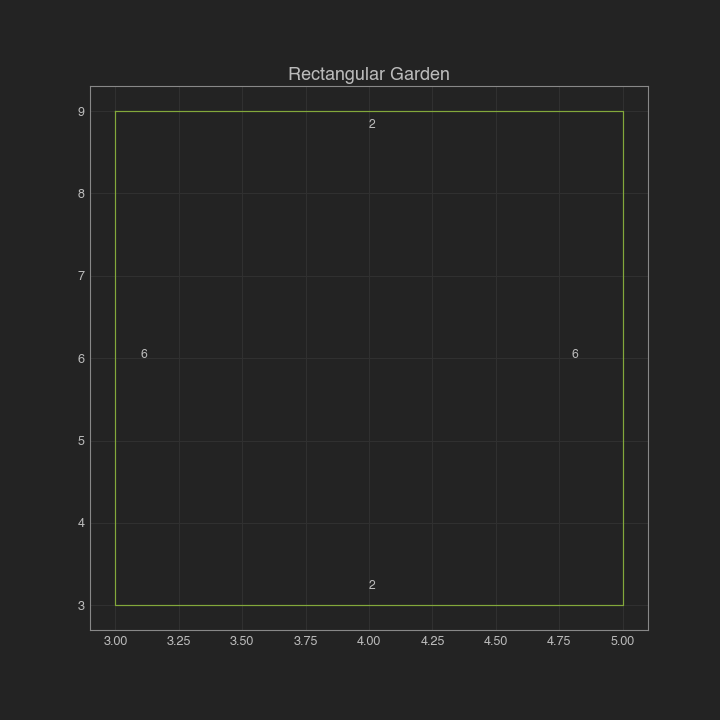
\includegraphics[width=1.0\columnwidth]{q37_figure}
    \caption{Rectangular Garden}
  \end{figure}
  \par
  To find out how much mulch is needed to cover the garden, we first need to find out the area of the garden. Since we know the length and width, we can multiply them to get the area.
  \begin{align}
    A = lw \\
    A = 6 * 2 = 12 \\
  \end{align}
  \par
  Finally, we divide the area by the area covered by each bag to get the number of bags. Once we know the number of bags, we multiply by the price of each bag to get the final answer.
  \begin{align}
    12 / 5 = 2.40 \\
    3 * 5 = 15
  \end{align}
  The total cost will be \$ 15 since 3 total bags are needed to cover the entire area of the garden.
\end{center}
\end{document}
